% -------------------------------- PREAMBLE --------------------------------
\documentclass[a4paper]{report}

\usepackage[utf8]{inputenc}
\usepackage{graphicx}
\usepackage{tikz}
\usepackage{booktabs}
\usepackage[format=hang,font=small,labelfont=bf]{caption}
\usepackage[protrusion=true,expansion=true]{microtype}
\usepackage{amsmath}
\usepackage{amssymb}
\usepackage{amsthm}
\usepackage{upgreek}
\usepackage{nbaseprt}
\usepackage{appendix}
\usepackage{color}
\usepackage{url}
\usepackage{hyperref}
\usepackage{underscore}
\usepackage[numbers]{natbib}
\usepackage{enumitem}
\usepackage{algorithm}
\usepackage{algorithmicx}
\usepackage{algpseudocode}

\newcommand{\reporttitle}{Metric Based Data Analysis Techniques}
\newcommand{\reportauthor}{George Kettleborough}

% --- hyperref stuff ---
\definecolor{darkblue}{rgb}{0,0,0.4}
\hypersetup{
  pdftex,
  bookmarks=true,
  bookmarksopen=true,
  colorlinks=true,
  citecolor=black,
  filecolor=black,
  linkcolor=black,
  urlcolor=darkblue,
  pdfauthor={\reportauthor},
  pdftitle={\reporttitle},
  pdfsubject={}
}
\providecommand{\doi}[1]{\href{http://dx.doi.org/#1}{doi: #1}}

% --- TikZ stuff ---

\usetikzlibrary{calc,trees,positioning,arrows,chains,shapes.geometric,%
  decorations.pathreplacing,decorations.pathmorphing,shapes,%
  matrix,shapes.symbols}

% --- End TikZ stuff ---


% the figures location
\graphicspath{./figures/}

% make equations and figures numbered (sec.eq)
% \numberwithin{equation}{section}
% \numberwithin{figure}{section}

% new operators for maths
\DeclareMathOperator{\op}{op}
\DeclareMathOperator{\remainder}{remainder}
\DeclareMathOperator{\lc}{lc}
\DeclareMathOperator{\pquo}{pquo}
\DeclareMathOperator{\prem}{prem}
\DeclareMathOperator{\pp}{pp}
\DeclareMathOperator{\cont}{cont}
\DeclareMathOperator{\resultant}{resultant}
\DeclareMathOperator{\numerator}{numerator}
\DeclareMathOperator{\denominator}{denominator}
\DeclareMathOperator{\ADCO}{ADCO}
\DeclareMathOperator{\dens}{dens}
\DeclareMathOperator{\symdif}{\bigtriangleup}
\DeclareMathOperator*{\argmin}{arg\,min}
\DeclareMathOperator*{\tr}{tr}

\newcommand{\dset}{\mathcal{D}}
\newcommand{\clus}{\mathcal{C}}
\newcommand{\NP}{\text{NP}}

% theorems
\newtheorem{thm}{Theorem}
\newtheorem{lem}{Lemma}
\newtheorem{cor}{Corollary}
\newtheorem{dfn}{Definition}

% problem template
\newenvironment{problem}[1]{\par\addvspace{\topsep}\noindent\textsc{#1}\\}
{\par\addvspace{\topsep}}
\newcommand{\instance}[1]{\textsc{Instance:} #1\\}
\newcommand{\question}[1]{\textsc{Question:} #1}

\title{\reporttitle}
\author{\reportauthor}

% ------------------------------ END PREAMBLE ------------------------------

\begin{document}

\maketitle

\tableofcontents

\chapter{Introduction}
\label{cha:introduction}

\chapter{Background}
\label{cha:background}

\section{Summary}
\label{sec:summary-backgd}


\section{Datasets and metric spaces}
\label{sec:datas-metr-spac}

Let $M$ be a set and $d \colon M \times M \to \mathcal{R}$ a function where,
for all $x,y \in M$, the following conditions hold
\begin{enumerate}
\item $d(x,y) \geq 0$,
\item $d(x,y) = d(y,x)$,
\item
  \begin{enumerate}
  \item $d(x,x) = 0$.
  \end{enumerate}
\end{enumerate}
Such a function is called a distance and can be used to measure the similarity
between elements of $M$: closer elements are more similar and distant elements
less similar.  If we add two more conditions, namely, for all $x,y,z \in M$,
\begin{enumerate}[start=3]
\item
  \begin{enumerate}[start=2]
  \item $d(x,y) = 0$ only if $x=y$,
  \end{enumerate}

\item $d(x,y) + d(y,x) \geq d(x,z)$,
\end{enumerate}
then $d$ is also a \textit{metric} and the ordered pair $(M,d)$ is called a
\textit{metric space}.

A metric is the most intuitive type of dissimilarity measure for human use.
In a metric space, for example, if we know that some object $a$ is distant
from some object $b$, and we know that another object $c$ is close to $b$,
then it is natural for us to make the deduction that $c$ is also distant from
$a$.  This deduction would be incorrect in a general distance space.

A dataset is simply a collection of data.  These data usually arise as the
result of an experiment, for example the classic iris dataset arose from
measuring parts of certain flowers.  One of the first things one might wish to
do with such a dataset is compare its elements.

One way to do this is to invent a metric for the dataset.  If the elements are
of a common type, such as real valued vectors, then an existing metric can be
used, for example the well known Euclidean metric.

It is tempting to think of the dataset and some metric as a metric space, but
this is not strictly correct.  The reason is that, contrary to the name, a
dataset if not generally a set, but a multiset.  In other words, identical
elements can appear more than once.  We therefore define a dataset to be a
multiset $(\dset, \mu_{\dset})$ where $\dset$ is called the underlying set and
$\mu_{\dset} \colon \dset \to \mathbb{Z}^+$ is called the membership function
and maps each element of $\dset$ to its multiplicity.  If $d$ is a metric
defined for all elements in $\dset$, then $(\dset, d)$ is a metric space.

For the purposes of discussion we will only explicitly treat a dataset as a
multiset when it is necessary.  Normally we will just work on $\dset$ directly
and assume that $\mu_{\dset}(x) = 1$ for all $x \in \dset$.

\section{Partitions}
\label{sec:partitions}

In this section we look at the properties of partitions of datasets, how we
can compare partitions and how we can find partitions.

\subsection{The space of partitions}
\label{sec:space-partitions}

A partition of a (multiset) dataset, $(\dset,\mu_{\dset})$, is a set of $k$
multisets, $\{(C_1,\mu_1),(C_2,\mu_2),\dotsc,(C_k,\mu_k)\}$ where $C_1 \cup
C_2 \cup \dotsb \cup C_k = \dset$, for all $i = 1,\dotsc,k, \sum_{x \in \dset}
\mu_i(x) > 0$ and, for all $x \in \dset$, $\sum_{i=1}^{k} \mu_i(x) =
\mu_{\dset}(x)$.  In other words, it is a set of nonempty, nonoverlapping
subsets.  These subsets are called clusters.

\begin{figure}
  \centering
  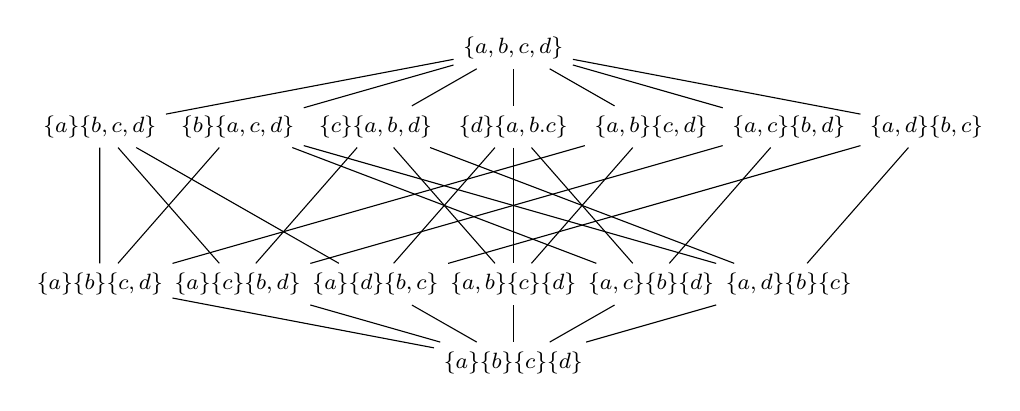
\begin{tikzpicture}[
    xscale=1.75, font=\footnotesize]

    % vertices
    
    \node (0) at (0,0) {$\{a,b,c,d\}$};

    \node (10) at (-3,-1) {$\{a\}\{b,c,d\}$};
    \node (11) at (-2,-1) {$\{b\}\{a,c,d\}$};
    \node (12) at (-1,-1) {$\{c\}\{a,b,d\}$};
    \node (13) at (0,-1) {$\{d\}\{a,b.c\}$};
    \node (14) at (1,-1) {$\{a,b\}\{c,d\}$};
    \node (15) at (2,-1) {$\{a,c\}\{b,d\}$};
    \node (16) at (3,-1) {$\{a,d\}\{b,c\}$};

    \node (20) at (-3,-3) {$\{a\}\{b\}\{c,d\}$};
    \node (21) at (-2,-3) {$\{a\}\{c\}\{b,d\}$};
    \node (22) at (-1,-3) {$\{a\}\{d\}\{b,c\}$};
    \node (23) at (0,-3) {$\{a,b\}\{c\}\{d\}$};
    \node (24) at (1,-3) {$\{a,c\}\{b\}\{d\}$};
    \node (25) at (2,-3) {$\{a,d\}\{b\}\{c\}$};

    \node (3) at (0,-4) {$\{a\}\{b\}\{c\}\{d\}$};

    % edges

    \draw (0) to (10);
    \draw (0) to (11);
    \draw (0) to (12);
    \draw (0) to (13);
    \draw (0) to (14);
    \draw (0) to (15);
    \draw (0) to (16);

    \draw (10) to (20);
    \draw (10) to (21);
    \draw (10) to (22);
    \draw (11) to (20);
    \draw (11) to (24);
    \draw (11) to (25);
    \draw (12) to (21);
    \draw (12) to (23);
    \draw (12) to (25);
    \draw (13) to (22);
    \draw (13) to (23);
    \draw (13) to (24);
    \draw (14) to (20);
    \draw (14) to (23);
    \draw (15) to (21);
    \draw (15) to (24);
    \draw (16) to (22);
    \draw (16) to (25);

    \draw (20) to (3);
    \draw (21) to (3);
    \draw (22) to (3);
    \draw (23) to (3);
    \draw (24) to (3);
    \draw (25) to (3);
  \end{tikzpicture}
  \caption{The lattice of partitions of dataset $\{a,b,c,d\}$ \citep{meila-2005}.}
  \label{fig:lattice}
\end{figure}

Let $\mathcal{P}_{\dset}$ be the set of all partitions of $\dset$.  The
natural way to represent the set $\mathcal{P}_{\dset}$ is as a graph called
the lattice of partitions.  Such a graph is shown in figure~\ref{fig:lattice}.
The top of the graph contains a single node containing $\hat{1} = \{\dset\}$
which is the partition with one cluster and the bottom is a single node
containing $\hat{0} = \{\{D_1\},\{D_2\},\dotsc,\{D_n\}\}$ the partition
containing $n$ clusters.

A partition, $\clus'$, which is obtained by splitting one or more clusters in
$\clus$ is said to be a refinement of $\clus$.  Every edge in the lattice
represents a refinement, with the coarser partition at the top.

As can be seen from figure~\ref{fig:lattice}, the number of possible
partitions for a 4 element dataset is already quite large; for a 20 element
dataset the number is more than 51 trillion.  In general the number of
possible partitions of an $n$ element dataset is equivalent to the $n$th Bell
number, $B_n$~\citep{bell1934exponential}.  The sequence of Bell numbers
begins with $B_0 = 1$ and its growth is then superexponential in $n$.  The
rest of sequence can be generated in a few ways including by a recursive
formula:
\begin{equation*}
  B_n = \sum_{k=0}^{n-1} B_k {n-1 \choose k},
\end{equation*}
or using Dobinski's formula:
\begin{equation*}
  B_n = \frac{1}{e} \sum_{k=0}^{\inf} \frac{k^n}{k!}.
\end{equation*}

\subsection{Comparing partitions}
\label{sec:comparing-partitions}

Since the space of possible partitions for any given dataset is very large, it
becomes useful to speak of similarity between different partitions.  It is
highly likely that different clustering algorithms will produce different
partitions given the same dataset, and some algorithms are non-deterministic,
for example $k$-means is often ``seeded'' with random clusters.  Such a
(dis)similarity measure could therefore be used to compare algorithms, or
assess the ability of a non-deterministic algorithm to consistently find good
solutions for hard problems.

It is quite easy to devise dissimilarity measures for partitions, but those
that are generally found most useful are distances, meaning they satisfy
conditions 1--3 of the metric definition.  If a dissimilarity measure further
satisfies condition~4 then it is also a metric.  A metric is the most
intuitive type of measure for human use.  In a metric space, for example, if
we know that some object $a$ is distant from some object $b$, and we know that
another object $c$ is close to $b$, then it is natural for us to make the
deduction that $c$ is also distant from $a$.  This deduction would be
incorrect in a general distance space.

We would argue that metrics are therefore the most desirable type of
dissimilarity measure.  Many metrics have been devised, and many more measures
that are not metrics or not even distances.  Existing measures fall into four
main categories which will each be discussed in the following subsections.
Briefly, these are:
\begin{description}
\item[Pair counting] which counts pairs of data points to measure the
  ``agreement'' and ``disagreement'' between two clusterings,
\item[Set matching] which matches clusters in one clustering to clusters in
  the other and measures the difference between these matched pairs,
\item[Information theoretic measures] which use information theory to
  describe the mutual information between two clusterings,
\item[Density profile based measures] which takes into account the attributes
  of the data set when determining similarity between clusterings.
\end{description}

As usual, let $\mathcal{D} = \{D_1,D_2,\dotsc,D_n\}$ be our data set and $P_1
= \{C_{11},C_{12},\dotsc,C_{1k}\}$ and $P_2 =
\{C_{21},C_{22},\dotsc,C_{2k'}\}$ be two partitions of $\mathcal{D}$.  The
contingency matrix of $P_1$ and $P_2$ is a $k \times k'$ matrix where the
$ij$-th element is $n_{ij} = |C_{1i} \cap C_{2j}|$.

\subsubsection{Pair counting}
\label{sec:pair-counting}

There are $\binom{n}{2}$ distinct pairs of objects in $\mathcal{D}$, and these
can be divided into four types:
\begin{description}
\item[$N_{11}$]: objects which are in the same cluster in $P_1$ and in the
  same cluster in $P_2$,
\item[$N_{00}$]: objects which are in different clusters in $P_1$ and in
  different clusters in $P_2$,
\item[$N_{10}$]: objects which are in the same cluster in $P_1$ but in
  different clusters in $P_2$,
\item[$N_{01}$]: objects which are in different clusters in $P_1$ but in the
  same cluster in $P_2$.
\end{description}

$N_{11}$ and $N_{00}$ are considered to be ``agreements'' and $N_{10}$ and
$N_{01}$ are ``disagreements''.  Clearly $N_{11} + N_{00} + N_{10} + N_{01} =
\binom{n}{2}$ is always satisfied.  The four counts can be obtained from the
confusion matrix \citep{fowlkes-mallows-1983}.

There are a number of different criteria that have been used in the literature
that are based on these counts.  The simplest of these are
$\mathcal{R}(P_1,P_2) = (N_{11}+N_{00})/\binom{n}{2}$ used by
\citet{rand-1971}; $(N_{10}+N_{01})/\binom{n}{2}$ used by Johnson, Mirkin,
Arabie and Boorman; and $(N_{11}+N_{00}-N_{10}-N_{01})/\binom{n}{2}$ used by
Hubert \citep{hubert-arabie-1985}.  The first of these, known as the Rand
index, is widely used and often cited in the literature.

\citet{fowlkes-mallows-1983} present a measure which they call $B_k$ for
comparing two hierarchical clusterings.  \citet{wallace-1983} later showed
that this measure could be stated in terms of two asymmetric measures
\begin{equation*}
  \mathcal{W}_{I}(P_1,P_2) = \frac{N_{11}}{\sum_{i=1}^{k}
    |C_{1i}|(|C_{1i}|-1)/2}
\end{equation*}
and
\begin{equation*}
  \mathcal{W}_{II}(P_1,P_2) = \frac{N_{11}}{\sum_{j=1}^{k'}
    |C_{2j}|(|C_{2j}|-1)/2},
\end{equation*}
which represent the probabilities that a pair of points which are in the same
cluster in $P_1$ and $P_2$ respectively, are also in the same cluster in the
other partition.  It was shown that Fowlkes and Mallows's original symmetric
measure is then simply the geometric mean of these two asymmetric measures
\citep{wallace-1983}
\begin{equation*}
  \mathcal{F}(P_1,P_2) = \sqrt{\mathcal{W}_{I}(P_1,P_2)\mathcal{W}_{II}(P_1,P_2)}.
\end{equation*}

The Jaccard coefficient \citep{ben-hur-2001} is an improved version of the
Rand index which is also well known and widely used
\begin{equation*}
  \mathcal{J}(P_1,P_2) = \frac{N_{11}}{N_{01}+N_{10}+N_{11}}.
\end{equation*}

So far, none of the measures listed are claimed to be metrics.  The Rand index
is clearly not a metric as it takes the value of $1$ for identical
clusterings.  In fact, the value of $N_{11}$ can always take a nonzero value
for identical clusterings.  Therefore both $\mathcal{F}$ and $\mathcal{J}$ are
not metrics as they are based on normalising the value of $N_{11}$.

One measure based on pair counting which is a metric is the Mirkin metric
\citep{mirkin-1996}
\begin{equation*}
  \mathcal{M}(P_1,P_2) = \sum_{i=1}^{k} |C_{1i}|^2 + \sum_{j=1}^{k'} |C_{2j}|^2
  - 2 \sum_{i=1}^{k} \sum_{j=1}^{k'} n_{ij}^2.
\end{equation*}
This can also be written as
\begin{equation*}
  \mathcal{M}(P_1,P_2) = 2(N_{01} + N_{10}) = n(n-1)(1-\mathcal{R}(P_1,P_2))
\end{equation*}
and is therefore an adjusted form of the Rand index \citep{meila-2007}.  In
fact, it turns out that the Rand index has been independently rediscovered in
different forms by many different authors \citep{hubert-arabie-1985}.

\subsubsection{Set matching}
\label{sec:set-matching}

These measures are based on the cardinality of the intersect of ``matched''
clusters.  \citet{meila-2001} present a method which finds a matching using a
heuristic: the greatest value in the contingency table, $n_{ab}$, is taken as
the first match, then the greatest value not in either row $a$ or column $b$
is the second match, and so on.  The function $match(i)$ gives the index of
the cluster in $P_2$ which matches cluster $C_{1i}$ by this heuristic.  The
measure is then
\begin{equation*}
  \mathcal{H}(P_1,P_2) = \frac{1}{n} \sum_{j=match(i)} n_{ij}.
\end{equation*}
A second measure used by \citet{larsen-aone-1999} is
\begin{equation*}
  \mathcal{L}(P_1,P_2) = \frac{1}{k} \sum_{i=1}^{k} \max_{j}
  \frac{2n_{ij}}{|C_{1i}|+|C_{2j}|}.
\end{equation*}
Neither of these are metrics.

The following was introduced by \citet{van-dongen-2000} and is a metric
\begin{equation*}
  \mathcal{D}(P_1,P_2) = 2n - \sum_{i=1}^{k} \max_{j} n_{ij} - \sum_{j=1}^{k'}
  \max_{i} n_{ij}.
\end{equation*}

\citet{meila-2005} introduces another metric called classification error which
they define as
\begin{equation*}
  d_{CE}(P_1,P_2) = 1 - \frac{1}{n} \max_{\sigma} \sum_{i=1}^{K} n_{i\sigma(i)}
\end{equation*}
where $K = \min(k,k')$.  Calculation of this metric requires finding a maximum
matching which can be done in polynomial time.  This metric is bounded by
$[0,1]$ but it ignores $k-k'$ clusters whenever $k>k'$ and vice versa.  The
proof that it is a metric is not provided in the paper.

\citet{meila-2007} points out that all of these measures suffer from the
so-called ``problem of matching''.  Given a clustering $P_1$ we can obtain a
second clustering $P_2$ by moving a fraction $f$ of the objects from each
cluster $C_i$ to $C_{(i+1)\bmod k}$.  We then obtain a third clustering $P_3$
from $P_1$ by reassigning the same fraction $f$ of objects from each cluster
evenly among the other clusters.  It is claimed that $P_3$ is intuitively a
less disrupted version of $P_1$ than $P_2$ is, but $\mathcal{H}(P_1,P_2) =
\mathcal{H}(P_1,P_3) = \mathcal{L}(P_1,P_2) = \mathcal{L}(P_1,P_3) =
\mathcal{D}(P_1,P_2) = \mathcal{D}(P_1,P_3)$ whenever $f < \frac{1}{2}$.

A similar problem is pointed out in \citet{bae-2010}.  However, it appears
that utilising the underlying metric space of the data would alleviate this
problem, but this is not discussed in the literature.

\subsubsection{Information theoretic}
\label{sec:inform-theor}

Two measures which use information theory are Normalized Mutual Information
(NMI) \citep{fred-jain-2003} and Variation of Information (VI)
\citep{meila-2007}.  These measures essentially show how much information one
clustering contains about the other \citep{bae-2010}.

\citet{meila-2005} compares some of these methods by viewing all possible
partitions of a data set as a lattice.  Five axioms are introduced which are
satisfied by VI.  Other methods are shown to satisfy some of these axioms.
A distance measure is said to ``align'' with the lattice if the distances can
be expressed in terms of a sum of distances along the edges of the lattice.
VI is shown to align with the lattice while classification error is shown to
be not aligned.

The variation of information is based on both how much information is
contained in each clustering and how much information one clustering contains
about the other.  The entropy associated with a clustering $P_1$ is defined as
\begin{equation*}
  H(P_1) = - \sum_{i=1}^{k} P_1(i) \log P_1(i)
\end{equation*}
where
\begin{equation*}
  P_1(i) = \frac{|C_{1i}|}{k} \quad \text{for $i = 1, \dotsc, k$}
\end{equation*}
which is the probability that an object picked randomly from $\mathcal{D}$
belongs to cluster $C_{1i}$.  The entropy tells us the uncertainty about which
cluster an object in $\mathcal{D}$ belongs to.

The mutual information between two clusterings, $P_1$ and $P_2$, is defined as
\begin{equation*}
  I(P_1,P_2) = \sum_{i=1}^{k} \sum_{j=1}^{k'} P_{12}(i,j)
  \log \frac{P_{12}(i,j)}{P_{1}(i) P_{2}(j)}
\end{equation*}
where
\begin{equation*}
  P_{12}(i,j) = \frac{|C_{1i} \cap C_{2j}|}{n}
\end{equation*}
which is the probability that an object picked randomly from $\mathcal{D}$ is
in both $C_{1i}$ in $P_1$ and $C_{2j}$ in $P_2$.

Variation of information is then defined as
\begin{equation*}
  VI(P_1,P_2) = H(P_1) + H(P_2) - 2I(P_1,P_2).
\end{equation*}
This is a metric \citep{meila-2007}.  It is also $n$-invariant which means it
depends only on the relative sizes of the clusters, not on the number of
objects in $\mathcal{D}$.

The metric is bounded for all $n$ by
\begin{equation*}
  VI(P_1,P_2) \leq \log n.
\end{equation*}
Also, if the number of clusters in each partition is at most $k^{*}$, where
$k^{*} \leq \sqrt{n}$ then the following bound is attained
\begin{equation*}
  VI(P_1,P_2) \leq 2 \log k^{*}.
\end{equation*}

\subsubsection{Density based}
\label{sec:density-based}

So far none of the measures we have seen have taken into account the
attributes of the data set, or that the data set itself is a metric space.
The Attribute Distribution Clustering Orthogonality (ADCO) measure uses
density profiles based on the attributes of the data set to measure the
similarity between clusterings \citep{bae-2010}.  This solves a few problems
with other techniques including the ``problem of matching'' mentioned in
section~\ref{sec:set-matching}.

To compute the measure, first each attribute of the data set is split into the
same number of bins.  Then a density profile vector is created for each
clustering based on the number of objects in each bin belonging to each
cluster.  The measure then takes the dot-product of one vector and a
transformation of the other vector.  The transformation is performed by a
maximum assignment function which is computed using the Hungarian algorithm in
$O(K_{\min}^3)$ time, where $K_{\min} = \min(k,k')$ \citep{bae-2010}.

The $\ADCO$ function itself is a non-negative similarity measure which takes a
higher value when clusterings are more similar.  This can be converted into a
distance measure defined as
\begin{equation*}
  D_{\ADCO}(P_1,P_2) =
  \begin{cases}
    2 - \ADCO(P_1,P_2) & \qquad \text{if $P_1 \neq P_2$},\\
    0 & \qquad \text{otherwise}.
  \end{cases}
\end{equation*}
The first case is true whenever the density profile vectors of each clustering
are not equal.  $D_{\ADCO}$ is a metric \citep{bae-2010}.

\section{Partional clustering}
\label{sec:part-clust-algor}

The problem of finding meaningful partitions of a dataset is called
partitional clustering.  In the following subjection we will discuss the
motivation for clustering and just a few of its many applications.  Then we
will discuss the problem itself which is broadly divided into two parts: first
one must decide what a meaningful partition actually is, and for this many
criteria have been suggested, and then one can attempt to find a good
partition according to that criterion.

\subsection{Motivation}
\label{sec:part-clus-motivation}

Broadly speaking, the applications of partitional clustering fall into two
categories: data reduction and object classification.

Data reduction may be desirable when a dataset is large and it is deemed that
only an essence of the data is necessary for the statistical precision
required.  If the data is to be displayed graphically to a user then an
overwhelmingly large dataset may not be desirable.  One real-world application
of data reduction in the latter category is the display of geographical data
on an electronic map.  By applying clustering, nearby elements can be grouped
to reduce clutter on the map.

Object classification finds applications in many fields including the natural
sciences, marketing and economics, computer science and engineering.  Given a
dataset obtained by market research one may wish to find different classes of
consumers in order to observe their habits and predict future behaviour.
Document clustering is an important area concerned with clustering on datasets
consisting of objects written in a natural language.  Search engines such as
those found on the World Wide Web use clustering to suggest ``similar''
documents to the one the user is currently interested in, amongst other things
\citep{steinbach2000comparison}.

\subsection{Complexity Issues}
\label{sec:complexity-issues}



\subsection{Criteria}
\label{sec:criteria}

Informally, a good partition of a dataset is one where the clusters are
homogeneous---meaning objects belonging to the same cluster are similar---and
well-separated---meaning objects belonging to different clusters are
dissimilar.

The task of judging a particular cluster based on these informal standards is
often a highly subjective one but, nevertheless, many objective criteria have
been devised for the purposes of automatic clustering.  It is the job of a
partitional clustering algorithm to find the globally optimal solution, which
means either the minimum or maximum according to a particular criterion.

We begin with a non-exhaustive list (from \citep{hansen1997mathprog}) of the
most general of criteria---those which only require a matrix if
dissimilarities between pairs of elements to compute them.  Let $\dset =
\{x_1,x_2,\dotsc,x_n\}$ be a dataset, $\clus = \{C_1,C_2,\dotsc,C_k\}$ be a
partition of $\dset$ and $d$ a dissimilarity measure on the elements of
$\dset$.  For the following criteria we do not need to know the values of the
elements of $\dset$, or how $d$ is computed, we only need the $n \times n$
dissimilarity matrix constructed by $d$.

The following criteria measure the homogeneity of a particular cluster,
$C_i$.  The diameter is the maximum dissimilarity between two members of the
cluster:
\begin{equation*}
  \max_{x,y \in C_i} d(x,y).
\end{equation*}
The radius is the minimum of the maximum dissimilarities between each member
and another member of the cluster:
\begin{equation*}
  \min_{x \in C_i} \max_{y \in C_i} d(x,y).
\end{equation*}
The star is the minimum of the sums of dissimilarities between each member
and every other member of the cluster:
\begin{equation*}
  \min_{c \in C_i} \sum_{x \in C_i} d(x,c).
\end{equation*}
The clique is the sum of dissimilarities between each pair of members of the
cluster:
\begin{equation*}
  \sum_{x,y \in C_i} d(x,y).
\end{equation*}

The following criteria measure the separation of a cluster, $C_i$, from every
other cluster.  The split is the maximum dissimilarity between a member of the
cluster and an element outside of the cluster:
\begin{equation*}
  \min_{x \in C_i, y \in \dset \setminus C_i} d(x,y).
\end{equation*}
The cut is the sum of dissimilarities between all members of the cluster and
all elements outside of the cluster:
\begin{equation*}
  \sum_{x \in C_i} \sum_{y \in \dset \setminus C_i} d(x,y).
\end{equation*}

Criteria for whole partitions could then be simply the sum over all partitions
of one of these criteria.  We call them sum-of-diameters, sum-of-radii,
sum-of-stars and so on.  Alternatively one could simply take the maximum or
minimum value, as appropriate, over the clusters which we would call
max-diameter, max-radius, min-cut and so on.  Clearly one would wish to
minimise the criteria for homogeneity and maximise those for separation.

Some criteria for homogeneity are equivalent to criteria for separation.  Most
notably, minimising sum-of-cliques is equivalent to maximising sum-of-cuts.
Such a criterion is therefore a criterion for both homogeneity and separation.

If the dataset is actually embedded in $m$-dimensional Euclidean space then
the following criteria based on the scatter or dispersion matrix of
\citet{wilks60} are possible.  The total scatter matrix for $\dset$ is a $m
\times m$ matrix defined
as:
\begin{equation*}
  \mathbf{T} = \sum_{i=1}^{k} (x_i - \bar{x})(x_i - \bar{x})^{\mathrm{T}}
\end{equation*}
where $\bar{x}$ is the mean value of $\dset$.  Two further matrices are
the within-cluster scatter matrix, $\mathbf{W} = \sum_{i=1}^{k} \mathbf{W}_i$,
where $\mathbf{W}_i$ is the scatter matrix for cluster $C_i$, and between
cluster scatter matrix
\begin{equation*}
  \mathbf{B} =
  \sum_{i=1}^{k} |C_i| (c_i - \bar{x}) (c_i - \bar{x})^{\mathrm{T}}
\end{equation*}
where $c_i$ is the mean of cluster $C_i$.  These matrices are related by the
equality
\begin{equation*}
  \mathbf{T} = \mathbf{W} + \mathbf{B}.
\end{equation*}

One possible criterion is the minimisation of the trace of $\mathbf{W}$.  This
is equivalent to minimising the trace of $\mathbf{B}$ since
\begin{equation*}
  \tr(\mathbf{T}) = \tr(\mathbf{W}) + \tr(\mathbf{B})
\end{equation*}
and $\mathbf{T}$ is a constant.  This criterion is actually equivalent to
minimising the sum over all clusters of the sum of Euclidean distances squared
between each member of the cluster and its centroid:
\begin{equation}
  \label{eq:tr(W)}
  \tr(\mathbf{W}) = \sum_{i=1}^{k} \sum_{x \in C_i} d^2(x,c_i),
\end{equation}
where $d$ is the Euclidean distance.  This can be seen easily by examining the
main diagonal of each $\mathbf{W}_i$:
\begin{multline*}
  \mathbf{W}_i = \\
  \sum_{x \in C_i}
  \begin{bmatrix}
    (x_1-c_{i1})^2 & (x_1-c_{i1})(x_2-c_{i2}) & \cdots &
    (x_1-c_{i1})(x_m-c_{im}) \\
    (x_2-c_{i2})(x_1-c_{i1}) & (x_2-c_{i2})^2 & \cdots &
    (x_2-c_{i2})(x_m-c_{im}) \\
    \vdots & \vdots & \ddots & \vdots \\
    (x_m-c_{im})(x_1-c_{i1}) & (x_m-c_{im})(x_2-c_{i2}) & \cdots &
    (x_m-c_{im})^2
  \end{bmatrix}
\end{multline*}
where $x_j$, $c_{ij}$ mean the $j$th component of $x,c_{i}$ respectively.

Similarly, maximising $\tr(\mathbf{B})$ is equivalent to maximising the sum of
Euclidean distances squares between each cluster centroid and $\bar{x}$,
multiplied by the cluster's cardinality:
\begin{equation}
  \label{eq:tr(B)}
  \tr(\mathbf{B}) = \sum_{i=1}^{k} |C_i| d^2(c_i,x).
\end{equation}
For this reason, this criterion is often called ``sum-of-squares'', although
this name is ambiguous since any criterion utilising sums of distances squared
could have this name.  We therefore call it centroid-distance, due to
measuring the distances between elements and centroids, and in general call
any criterion using sums of distances squared a sum-of-squares criterion.
Note that when centroid-distance is calculated using
equation~\eqref{eq:tr(W)}, we can use any metric for $d$.  If it is calculated
using the scatter matrix then it is implicitly using the Euclidean metric.

The relationship between equations~\eqref{eq:tr(W)} and \eqref{eq:tr(B)} can
also be shown by the Huygens-Steiner, or parallel-axis, theorem, which states
that
\begin{equation}
  \label{eq:huygens}
  \sum_{x \in C_i} d^2(x,s) = d^2(c_i,s) \dot |C_i| + \sum_{x \in C_i} d^2(x,c_i)
\end{equation}
where $s$ and the members of $C_i$ are in Euclidean space and $d$ is the
Euclidean distance.

We can also use this theorem to show a relationship between centroid-distance
and sum-of-cliques.  Beginning with equation~\eqref{eq:huygens} we assign some
$y \in C_i$ to $s$ and sum over all $y \in C_i$:
\begin{equation*}
  \sum_{x,y \in C_i} d^2(x,y) = \sum_{y \in C_i} d^2(c_i,y) \dot |C_i|
                           + \sum_{x \in C_i} d^2(x,c_i) \dot |C_i|
\end{equation*}
and, since $d$ is symmetric,
\begin{equation}
  \label{eq:cd-as-equivalence}
  \frac{\displaystyle \sum_{x,y \in C_i} d^2(x,y)}
       {|C_i|}
  = 2 \sum_{x \in C_i} d^2(x,c_i).
\end{equation}
So when we use Euclidean distance squared as dissimilarity measure,
centroid-distance for each cluster is equivalent to sum-of-cliques over twice
the cardinality of the cluster.  Since $d$ is symmetric this is the same as
only counting pairwise distances once each.

As mentioned, we generally call any criterion involving a metric squared a
sum-of-squares criterion.  We call the numerator of the left-hand side of
equation~\eqref{eq:cd-as-equivalence} all-squares, since we sum over all pairs
of distances.  Since sum-of-cliques can generally be used with any
dissimilarity measure we generally count each pair of elements twice, once in
each direction, but for a metric this is obviously redundant.

Two other criteria based on the scatter matrix, which were suggested by
\citet{friedman1967criteria}, are the minimisation of the determinant of
$\mathbf{W}$, sometimes called generalised variance, and the maximisation of
the trace of $\mathbf{BW}^{-1}$.  These criteria tend to produce clusters of
similar shape and size as centroid-distance with the Euclidean metric
\citep{marriott1982optimization}.

A further four criteria based on the scatter matrix are discussed in
\citep{marriott1982optimization}, these are
$\prod_{i=1}^{k}|\mathbf{W}_i|^{|C_i|}$, which is a generalisation of
$|\mathbf{W}|$ that allows cluster of different shapes,
$\sum_{i=1}^{k}|\mathbf{W}_i|^{\frac{1}{m}}$, introduced in
\citep{maronna1974}, $n \log{|\mathbf{W}|} - 2\sum_{i=1}^{k} |C_i|
\log{|C_i|}$ and $\sum_{i=1}^{k} (|C_i| \log{|\mathbf{W}_i|} -
2|C_i|\log{|C_i|})$.

All of the criteria based on the scatter matrix tend to produce ellipsoidal
clusters; clusters with other shapes will either not be found or be divided
into small clusters \citep{marriott1982optimization}.  Most of the criteria
also tend to produce clusters which are linearly-separable---meaning they are
separated by hyperplanes.

Some criteria are based on similarities instead of dissimilarities.  One such
example is the average entity stability of \citep{Rubin67optimal}.  This
criterion considers an object to be stable if it is more attracted to the rest
of the cluster it is currently in than to any other cluster.  Attraction to a
cluster is the average similarity between the object and the members of that
cluster.  The criterion is to maximise the average entity stability over the
whole dataset.

Criteria based on information theory are also possible.
\citet{wallace1968information} contains a clustering program called SNOB which
attempts to optimise one such information measure.

We finish our discussion on criteria with two further definitions.  The
partition which is the global minimum or maximum solution, whichever is
appropriate, for a particular criterion is called the optimal partition, for
example, we will later refer to the centroid-distance optimal partition,
all-squares optimal partition and so on.  The problem of finding an optimal
partition according to any criterion we will refer to simply as clustering,
and when we speak of a particular criterion we will say centroid-distance
clustering, all-squares clustering and so on.

\subsection{Methods}
\label{sec:methods}

Finding optimal clusterings according to any criteria is intuitively a hard
problem.  The problem of finding a centroid-distance optimal clustering was
assumed to be NP-complete for decades, although this was proved only
relatively recently\citep{aloise09exact}.  In
chapter~\ref{cha:sum-squar-clust} we show a more general proof of the
NP-completeness of centroid-distance clustering and show that all-squares is
NP-complete too.

The consequence of the complexity of the problem is that heuristic algorithms
for estimating optimal solutions are very prevalent.  Due to the ubiquity of
the clustering problem, a vast amount of literature has been generated on the
subject and a large number of different algorithms have been devised.  The
vast majority of clustering algorithms use heuristics with only a small
handful producing exact solutions.

\begin{algorithm}
  \caption{H-means, Lloyd's algorithm.}
  \label{alg:lloyds}
  
  \begin{algorithmic}
    \Require A dataset $\dset \subseteq M$, with $k$ means
    $\{c^0_1,c^0_2,\dotsc,c^0_k\} \subseteq M$.

    \ForAll{$1 \leq i \leq k$}
    \Comment{Initialise partition.}
       \State $C_i \gets \emptyset$
    \EndFor

    \ForAll{$x \in \dset$}
       \State $i \gets \argmin_{1 \leq j \leq k} d(x,c_j)$
       \State $C_i \gets C_i \cup \{x\}$
    \EndFor

    \State $n \gets 1$

    \Repeat
       \Comment{Update partition until means do not change.}
       
       \ForAll{$1 \leq i \leq k$}
       \Comment{Calculate new means.}
          \State $c^n_i \gets \min_{c \in M} \sum_{x \in C_i} d^2(x,c)$
       \EndFor

       \ForAll{$1 \leq i \leq k$}
          \Comment{Update partition.}
          \State $C_i \gets \emptyset$
       \EndFor
       
       \ForAll{$x \in \dset$}
          \State $i \gets \argmin_{1 \leq j \leq k} d(x,c_j)$
          \State $C_i \gets C_i \cup \{x\}$
       \EndFor

       \State $n \gets n+1$
       
       \Until{$\{c^{n-1}_1,c^{n-1}_2,\dotsc,c^{n-1}_k\} =
         \{c^{n-2}_1,c^{n-2}_2,\dotsc,c^{n-2}_k\}$}

          
       \State \Return{$\{C_1,C_2,\dotsc,C_k\}$}
  \end{algorithmic}
\end{algorithm}

The H-means algorithm for estimating the centroid-distance optimal
$k$-clustering is probably the most well-known and widely-used clustering
algorithm today.  It is also known as Lloyd's algorithm, although it was in
fact independently discovered by many different authors \citep{jain2010data},
and sometimes, confusingly, $k$-means, which is actually a different
algorithm.  Assuming that centroids are easy to compute, this algorithm is
simple and, generally, quickly converges to a local optimum.  However, in the
worst case, H-means requires exponentially many iterations in order to
converge on a solution, even in the Euclidean plane
\citep{vattani2009exponential}.

\begin{algorithm}
  \caption{$k$-means algorithm}
  \label{alg:k-means}

  \begin{algorithmic}
    \Require An initial $k$-clustering, $\clus = \{C_1,C_2,\dotsc,C_k\}$.

    \Repeat
       \State $\clus' = \{C'_1,C'_2,\dotsc,C'_k\} \gets \clus$
       \ForAll{$1 \leq l \leq k$}
          \ForAll{$x \in C'_l}$
             \ForAll{$m \in \{1,2,\dotsc,k\}\l$}
                \If{$\displaystyle
                  \frac{|C_m|}{|C_m|+1} d^2(x,c_m)
                  + \frac{|C_l|}{|C_l|-1} d^2(x,c_l) < 0$}
                   \State $C_l \gets C_l \ \{x\}$
                   \State $C_m \gets C_m \cup \{x\}$
                   \State $\phi \gets 1$
                \EndIf
             \EndFor
          \EndFor
       \EndFor
    \Until{$\phi=0$}
  \end{algorithmic}
\end{algorithm}



Some algorithms for exactly solving the centroid-distance problem are known
including methods using branch-and-bound \citep{brusco2006repetitive},
branch-and-cut \citep{aloise09exact} and column generation
\citep{merle1999interior}.  Some of these algorithms are able to exactly solve
instances in the plane of around 2000 elements in reasonable time
\citep{aloise09exact}.

The all-squares problem, or more generally sum-of-cliques, has received less
attention but there are, nonetheless, a number of algorithms described in the
literature.  An exact algorithm using branch-and-bound
\citep{klein1991optimal} can be used to solve problems with $n \leq 50, k \leq
5$ \citep{hansen1997mathprog}.  Cutting planes have also been applied with
problems with $n \leq 158$ solved quickly
\citep{hansen1997mathprog,palubeckis1997branch}.  In terms of heuristic
approaches, there is an obvious iterative agglomerative technique that can be
applied.  We have a simple randomised version that is showing some promise
\citep{gk2012agglomerative}.

\section{Hierarchies}
\label{sec:hierarchies}



\chapter{Sum-of-Squares Clustering}
\label{cha:sum-squar-clust}

\section{Summary}
\label{sec:summary-sum-squar}

This chapter is basically the paper I did with Vic.

\chapter{Tree Stuff}
\label{cha:tree-stuff}

\chapter{Further Work}
\label{cha:further-work}



\bibliographystyle{plainnat}
\bibliography{../comp-clustering.bib,../clustering.bib}

\end{document}
